%\documentclass[a4paper, openany, problemsheet, FlipAns]{TsangPS}
\documentclass[a4paper, openany, solutions, FlipAns]{TsangPS}


\unittitle{Vibrations, Waves, and Optics}
\unitcode{PHYS10005/53}
\lecturer{D. Tsang \& A. Narduzzo}
\setnumber{2}
\logo[-0.5cm]{uob_logo.pdf}
\semester{Semester I --- 2018/2019}
\date{Due: 15 Oct 2018}% to remove date just set \date{}
\begin{document}
\maketitle

\begin{question}{The H.M.S. S.H.M.}{2}{1}{0}
\newq{A boat at anchor bobs} up and down with the waves. The boat moves 5 cm above and 5 cm below its equilibrium position, and makes one complete up-and-down cycle every 4 s. What are the amplitude, period, frequency, and angular frequency of the motion?

\solution{
The amplitude is $\boxed{A = 5\,{\rm cm}}$, and the period is $\boxed{T=4\,{\rm s}}$.
\marginnote{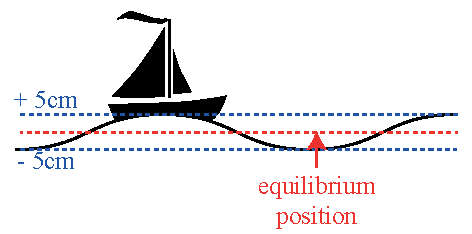
\includegraphics{Q1_Boat.pdf}}
The frequency and angular frequency are given by
\begin{align*}
\Aboxed{f &= \frac{1}{T} = \frac{1}{4\, {\rm s}} = 0.25\, {\rm Hz}}\\
\Aboxed{\omega &= 2\pi \times f = 2\pi \times 0.25\, {\rm Hz} = 1.57\, {\rm rad}/{\rm s}}
\qed
\end{align*}
}{5 cm, 4 s, 0.25 Hz, 1.57 rad/s}
\end{question}

\makeline

\end{document}